\documentclass[11pt,a4paper,openright,twoside]{report}

\usepackage[british]{babel}
\usepackage[utf8]{inputenc}

\usepackage{fancyhdr}
\usepackage{indentfirst}
\usepackage{graphicx}
\usepackage{newlfont}
\usepackage{xcolor}
\usepackage{stmaryrd}


\usepackage{amssymb}
\usepackage{amsmath}
\usepackage{latexsym}
\usepackage{amsthm}


\oddsidemargin=25pt 
\evensidemargin=15pt
\hyphenation{pa-ra-me-tric}
\pagestyle{fancy}\addtolength{\headwidth}{20pt}
\renewcommand{\chaptermark}[1]{\markboth{\thechapter.\ #1}{}}
\renewcommand{\sectionmark}[1]{\markright{\thesection \ #1}{}}
\rhead[\fancyplain{}{\bfseries\leftmark}]{\fancyplain{}{\bfseries\thepage}}
\cfoot{}
\linespread{1}

% Style theorem boxes

\theoremstyle{plain}
\newtheorem{proposition}{Proposition}
\newtheorem{definition}[proposition]{Definition}

\theoremstyle{definition}
\newtheorem{remark}[proposition]{Remark}
\newtheorem{example}[proposition]{Example}


%%%%%%%%%%%%%%%%%%%%%%%%% DEDICATION %%%%%%%%%%%%%%%%%%%%%%%%%%%%%%%%%%%%%%%

\begin{document}

\begin{titlepage}
\thispagestyle{empty}                   
\topmargin=6.5cm                        
\raggedleft                             
\large                                  
                                       
\em                                     
To my beloved\\
Benedetta                   
\newpage                                

\clearpage{\pagestyle{empty}\cleardoublepage}
\end{titlepage}
\pagenumbering{roman}


            




%%%%%%%%%%%%%%%%%%%%%%% INTRODUCTION %%%%%%%%%%%%%%%%%%%%%%%%%%%%%%

\chapter*{Introduction}   
\addcontentsline{toc}{chapter}{Introduction}
\rhead[\fancyplain{}{\bfseries Introduction}]{\fancyplain{}{\bfseries\thepage}}\lhead[\fancyplain{}{\bfseries\thepage}]{\fancyplain{}{\bfseries Introduction}}



  \section*{English version}




  \textcolor{blue}{Machine learning literature is exploding in size and complexity, but most solutions found are ad hoc, there is little communication between different subfields, and there is a large research debt. Category theory can solve these problems.  \cite{shieblerCategoryTheoryMachine2021}.}

  \textcolor{blue}{Talk about the origins of category theory and its "rise to power" as a common language that aims to unite different fields of knowledge.}
    
  \textcolor{blue}{Discuss the purpose of this work: a beginner-friendly survey of categorical approaches to neural networks, causal models, and interpretability.}


  \section*{Italian version}

  \textcolor{blue}{Traduzione italiana dell'introduzione.}


\clearpage{\pagestyle{empty}\cleardoublepage}


%%%%%%%%%%%%%%%%%%%%%%%%%%%%% TABLE OF CONTENTS %%%%%%%%%%%%%%%%%%%%%%%%%%%%%%

\tableofcontents
\rhead[\fancyplain{}{\bfseries\leftmark}]{\fancyplain{}{\bfseries\thepage}} \lhead[\fancyplain{}{\bfseries\thepage}]{\fancyplain{}{\bfseries Table of Contents}}
\clearpage{\pagestyle{empty}\cleardoublepage}


%%%%%%%%%%%%%%%%%%%%%%% CATEGORICAL APPROACHES TO NNS %%%%%%%%%%%%%%%%%%%%%%%%%%%


\chapter{Categorical Approaches to Neural Networks}
\lhead[\fancyplain{}{\bfseries\thepage}]{\fancyplain{}{\bfseries\rightmark}}
\pagenumbering{arabic}




\textcolor{blue}{Brief summary of the chapter. Take inspiration from \cite{abbottCategoryTheoryArtificial2024} in dividing the chapter into three parts: generic compositional frameworks, data representation learning, compositional architecture design.}




\section{General Compositional Frameworks for Neural Networks}



\subsection{Gradient-based Learning with Parametric Lenses}

\subsubsection{Parametric Lenses as a General Model}

Pretrained neural networks can be though of as differentiable functions between Euclidean spaces, but a more sophisticated model is needed if we want to study the training process in its entirety. A neural network that needs to be trained is best thought of as a parametric map: training means finding the best parameters for the task at hand. Thus, it makes sense to represent layers of a neural network as parametric maps in $(P,f) \in \mathbf{Para}(\mathcal{C})(A,B)$, for some symmetric monoidal category $\mathcal{C}$.


The process of training, however, requires a bidirectional flow of information: we have to test the current parameters and apply some criterion to find new parameters that (hopefully) satisfy the requirements better. In gradient based learning, the aforementioned criterion requires computing the gradient of the loss function using specialized algorithms such as backpropagation. It has been shown numerous time (see e.g. ADDREF) that taking the reverse derivative instead of the forward derivative is more efficient for functions with lower dimensionality in the codomain, which is commonplace in real word neural networks. Hence, it makes sense to require $\mathcal{C}$ to be CRDC. 

The position held by \cite{cruttwellDeepLearningParametric} is that the most natural way to relate forward and backward propagation of information in neural network is to represent the components of the network as parametric lenses where the get map handles forward propragation while the put map handles backward propagation. For instance,  in place of $(P,f)$, we would consider
\begin{equation}
  \label{eq: exparametriclens}
  \left(\begin{pmatrix} P \\ P \end{pmatrix},\begin{pmatrix} f \\ \mathrm{R}[f] \end{pmatrix}\right) 
  \in \mathbf{Para}(\mathbf{Lens}(\mathcal{C}))
  \left(\begin{pmatrix} A \\ A \end{pmatrix},\begin{pmatrix} B \\ B \end{pmatrix}\right).
\end{equation}
The authors of \cite{cruttwellDeepLearningParametric} take this line of reasoning a step further and show that it is also meaningful to represent other components of learning - such as optimizers, loss functions, and learning rates - within the framework of parametric lenses. 


The main insight that makes parametric lenses as the one above useful is contained in \textit{Prop. \ref{proposition: canembedding1}} and \textit{Prop. \ref{proposition: canembedding2}}. If $\mathcal{C}$ is CRDC, we can functorially embed $\mathcal{C}$ into $\mathbf{Lens}(\mathcal{C})$ by considering lenses whose put map is the reverse derivative of the get map. Moreover, we can functorially embed $\mathbf{Para}(\mathcal{C})$ into $\mathbf{Para}(\mathbf{Lens}(\mathcal{C}))$ with the same exact "trick". Hence, lenses as the one in \textit{Eq. \ref{eq: exparametriclens}} are compositional. In addition, (i) the get map of the composition of two lenses is the composition of the get maps, (ii) the put map of the composite lens is the reverse derivative of the composition of the put maps. Hence, if $\left(\left(\begin{smallmatrix} P \\ P \end{smallmatrix}\right),\left(\begin{smallmatrix} f \\ \mathrm{R}[f] \end{smallmatrix}\right)\right)$ represents a linear layer and $\left(\left(\begin{smallmatrix} Q \\ Q \end{smallmatrix}\right),\left(\begin{smallmatrix} g \\ \mathrm{R}[g] \end{smallmatrix}\right)\right)$ represents an activation layer, their composition represents a fully connected layer according to the same convention.


\subsubsection{Other Components Needed for Learning}


Surprisingly, even loss maps can be represented as parametric maps and thus as parametric lenses.
For instance, we may represent a loss maps as $(P,\mathrm{loss}) \in \mathbf{Para}(\mathcal{C})(B,L)$ for some object $L$. The intuitive meaning of this representation is the following: $\mathrm{loss}$ takes the output of the network of type $B$, compares it with the labels of type $P$ ($P$ and $B$ will often coincide in practical examples), and then returns a loss of type $L$. The parametric lens associated with $\mathrm{loss}$ can thus be post-composed after the parametric lens associated with a neural network to compute the loss generated by such network given some input and the associated labels. This process is illustrated in Fig. ADDIM.


This leaves two dangling wires of type $L$. We can use a learning rate lens $\alpha$ to link the wires and allow forward-propagating information to "change direction" and go backwards. $\alpha$ must have domain equal to $\left( \begin{smallmatrix} L \\ L \end{smallmatrix} \right)$ and codomain equal to $\left(\begin{smallmatrix} 1 \\ 1 \end{smallmatrix}\right)$, where $1$ is the terminal object of $\mathcal{C}$. For instance, if $\mathcal{C} = \mathbf{Smooth}$, $\alpha$ might just multiply the loss by some $\epsilon$, which is what machine learning practitioners would ordinarily call learning rate. Fig. ADDIM shows how a learning rate can be linked to the loss function and the model using post-composition.


The final element needed for the model $f$ in Fig. ADDIM to learn is an optimizer. It is shown in \cite{cruttwellDeepLearningParametric} that optimizers can be represented as reparametrisations in $\mathbf{Para}(\mathbf{Lens}(\mathcal{C}))$. More specifically, we might see an optimizer as a lens $\left( \begin{smallmatrix} P \\ P \end{smallmatrix} \right) \to \left( \begin{smallmatrix} Q \\ Q \end{smallmatrix} \right)$. In gradient descent, for example, $P = Q$ and the aforementioned lens is $\left( \begin{smallmatrix} 1_P \\ +_P \end{smallmatrix} \right)$. We can plug such reparametrisation on top of the model to obtain the string diagram in Fig. ADDIM. The diagram shows how the machinery hidden by the $\mathbf{Para}(\mathbf{Lens}(\mathcal{C}))$ can take care of forward propagation, loss computation, backpropagation and parameter updating in a seamless fashion. This is the true power of the compositional mindset: abstraction hides away unwanted detail so that one can focus on high-level features of the model without worrying about side-effects.


The authors of \cite{cruttwellDeepLearningParametric} go on to show that their compositional framework can handle a number of non-trivial deep learning architectures such as CNNs, GANs, and deep dreaming. For instance, the copy maps of CRDCs can model weight sharing and batching, and even a whole learning iteration can be represented as a large string diagram. Finally, the authors prove that the compositional point of view afforded by parametric lenses is of practical significance by implementing a proof-of-concept Python library. The library is then used to build a model able to classfy MNIST. In their words, \lq[the] proposed algebraic structures naturally guide programming practice\rq.


\subsubsection{Learners and Generalizations}

We have presented the perspective of \cite{cruttwellDeepLearningParametric} within the context of neural networks for the sake of simplicity, but the tools introduced in the paper apply to a much wider context. More precisely, lenses and parametric lenses can model any system trained according to a gradient-based learning algorithm, as long as such gradient is computed in the form of a reverse derivative in a CRDC.  For instance, it is shown in \cite{wilsonCategoriesDifferentiablePolynomial2022} that polynomial circuits form a CRDC, and it is shown in \cite{wilsonReverseDerivativeAscent2021a} that meaningful learning can be carried out in the context of Boolean circuits, as long as a suitable optimizer is chosen. Hence, the framework described in this section can be applied as is to Boolean circuits. Working in an abstract categorical setting allows for this kind of generality. 


One of the first compositional approaches to training neural networks in the literature can be found in the seminal paper \cite{fongBackpropFunctorCompositional2019a}. The authors introduce a category of learners, objects which are meant to represent components of a neural network and behave similarly as parametric lenses do. The main difference is that each learner is endowed with its own loss map and optimizer. It is argued in \cite{cruttwellDeepLearningParametric} and ADDREF that the perspective \cite{cruttwellDeepLearningParametric} is more flexible than and largely subsumes the learner approach. 


\section{Functor Learning}

In the parametric lens framework presented above, learning happens at the morphism level. The framework is very convenient because its categorical structure hides away the automatic differentiation machinery needed for backpropagation, and thus we can just compose the parametric lenses as modules, so that we can form any network we wish. However, parametric lenses cannot be used to abstract away computations and extract the schema of the model, as they inherently carry out computations. Moreover, the generality of the parametric lens framework means that no tools are developed to study and exploit the inherent structure of the data. Finally, parametric lenses do not offer high level tools to deal with invariance ad equivariance constraints. 

It has been suggested by \cite{gavranovicLearningFunctorsUsing2020} and \cite{sheshmaniCategoricalRepresentationLearning2022} that the key to link different layers of abstraction and to exploit the structure of the data is to learn functors instead of morphisms. \cite{gavranovicLearningFunctorsUsing2020} and \cite{vaswaniAttentionAllYou2023} also use functor learning to provide tools that implement abstract constraints on neural networks.



\subsection{Functors to Separate Layers of Abstraction}

The author of \cite{gavranovicLearningFunctorsUsing2020} takes inspiration from categorical data migration - a field which is located at the intersection of category theory and database theory - to create a categorical framework for deep learning that separates the development of a machine learning process into a number of key steps. The different steps operate on different levels of abstraction and are linked by functors.

\subsubsection{Schemas}

The first step in the learning pipeline proposed by \cite{gavranovicLearningFunctorsUsing2020} is to write down the bare-bones structure of the model in question. One can do that using a directed multigraph $G$, where nodes represent data and edges represent neural networks interacting with such data. Constraints can be added at this level in the form of a set $\mathcal{X}$ of equations that identify parallel paths (see e.g. ADDIM, whose multigraph represent a cycleGAN model).


We can now consider the most abstract categorical representation of such model: its schema. 

\begin{definition}[Model schema]
  The schema of a model represented by a multigraph $G$ is the freely generated category $\mathbf{Free}(G)$.
\end{definition}

Such schema does not contain any data nor does it do any computation, but it encodes the bare-bones structure of the model. We can take the module $\mathbf{Free}(G)/{\sim}$, where ${\sim}$ is the path congruence relation induced by the equations in $\mathcal{X}$. Depending on the context, the word schema will also refer to such constrained category.

\subsubsection{Architectures and models}


Given the schema $\mathbf{Free}(G)$, we can choose an architecture for the model. What we mean by choosing architecture is assigning to each node a Euclidean space and to each morphism a parametric map, which represents an untrained neural network.

\begin{definition}[Model architecture]
  Let $\mathrm{Free}(G)$ be a model schema. An architecture for such schema is a functor $\mathsf{Arch}: \mathrm{Free}(G) \to \mathbf{Para}(\mathbf{Smooth})$.
\end{definition}

The Euclidean spaces $\mathsf{Arch}$ maps objects to might be intuitively interpreted as the spaces the data will live in, but it is best to consider data outside the $\mathbf{Para}$ machinery and in the simpler $\mathbf{Set}$ category, as this allows for better compartmentalisation. Thus, \cite{gavranovicLearningFunctorsUsing2020} also defines an embedding functor, which agrees with $\mathsf{Arch}$ on objects but exists independently of it.


\begin{definition}[Model embedding]
  Let $\mathrm{Free}(G)$ be a model schema and let $\mathsf{Arch}$ be a chosen architecture. An embedding for such schema is a functor $E: |\mathrm{Free}(G)| \to \mathbf{Set}$ which agrees with $\mathsf{Arch}$ on objects\footnote{The reason why the domain $E$ is the discretised schema $|\mathrm{Free}(G)|$ instead of the original schema $\mathrm{Free}(G)$ will be clear once we define datasets.}.
\end{definition}

Consider the function $\mathfrak{p}: (P,f) \mapsto P$, which takes the parameter space out of a parametric map in $\mathbf{Para}(\mathbf{Smooth})$. We can use it to define a function 
\[\mathfrak{P}: \mathsf{Arch} \mapsto \prod_{f \in \mathsf{Gen}_{\mathbf{Free}(G)}}\mathfrak{p}(\mathsf{Arch}(f)),\]
where $\mathsf{Gen}_{\mathbf{Free}(G)}$ is the set of generating morphisms of the free category on the multigraph $G$. The function $\mathfrak{P}$ takes and architecture and returns the parameter space. Given $\mathfrak{P}$, we can define parameter specification function.

\begin{definition}[Parameter specification function]
  Let $\mathrm{Free}(G)$ be a model schema and let $\mathsf{Arch}$ be a chosen architecture. A parameter specification function is a function $\mathsf{PSpec}$ which maps a pair $(\mathsf{Arch}, p)$ - comprised of an architecture $\mathsf{Arch}$ and some $p \in \mathfrak{P}(\mathsf{Arch})$ - to a functor $\mathsf{Model}_p: \mathbf{Free}(G) \to \mathbf{Smooth}$. The functor $\mathsf{Model}_p$ takes the model schema and returns its implementation according to $\mathsf{Arch}$, partially applying $p_f$ to each $\mathsf{Arch}(f)$, so that we obtain an actual smooth map. 
\end{definition}

The functor $\mathsf{Model}_p$ can be seen as a bridge between the parametric notion of untrained neural network and the notion of neural network as a smooth map, which makes most sense after training. To better understand the relationship between $\mathsf{Arch}$ and $\mathsf{Model}_p$ see ADDIM.

\subsubsection{Datasets and concepts}

Now, if we hope to train the model we have defined, we will need a dataset. \cite{gavranovicLearningFunctorsUsing2020} suggests that a dataset should be represented as a subfunctor of the embedding functor:

\begin{definition}[Dataset]
  Let $E$ be a model embedding. Then, a dataset is a subfunctor $D_E: |\mathbf{Free}(G)| \to \mathbf{Set}$ which maps every object $A$ of the discretised free category to a finite subset $D_E(A) \subseteq E(A)$.
\end{definition}

\begin{remark}
  The reason why the author of \cite{gavranovicLearningFunctorsUsing2020} chooses to define $E$ and $D_E$ on discretised categories is because it often happens in practical machine learning that the available data is not paired. In these cases, it would be meaningless to provide an action on morphisms because they would end up being incomplete maps.
\end{remark}

Given a node $A$ of $G$, we have associated to $A$ a Euclidean space $E(A)$, e.g. $\mathbb{R}^n$, and a dataset $D_E(A)$. It makes sense to define another set $\mathfrak{C}(A)$ such that $D_E(A) \subseteq \mathfrak{C}(A) \subseteq E(A)$. A dataset may be considered a collection of instances of something more specific than just vectors; for instance, if we have a finite dataset of pictures of horses, we are clearly interested in the concept of horse, i.e. in the set of all possible pictures of horses, which is much larger than our dataset but still much smaller than the vector space used to host such pictures. The set $\mathfrak{C}(A)$ is the concept represented by $D_E(A)$: in the aforementioned example, $\mathfrak{C}(A)$ might be the set of all images representing horses. Hence, we can call $\mathcal{C}$ the concept functor. 

\begin{definition}[Concept functor]
  Given a schema $\mathbf{Free}(G)/{\sim}$, an embedding $E$ and a dataset $D_E$, a concept associated with this information is a functor $\mathfrak{C}: \mathbf{Free}(G)/{\sim} \to \mathbf{Set}$ such that, if $I: |\mathbf{Free}(G)| \to \mathbf{Free}(G)/{\sim}$ is the inclusion functor, $D_E \subseteq I;\mathfrak{C} \subseteq E$.
\end{definition}

As \cite{gavranovicLearningFunctorsUsing2020} states, $\mathfrak{C}$ is an idealization, but it is a useful idealization as it represent the goal of the optimization process: given a dataset $D_E: |\mathbf{Free}(G)| \to \mathbf{Set}$, we wish to learn the concept functor $\mathfrak{C}: \mathbf{Free}(G)/{\sim} \to \mathbf{Set}$. Total achievement of such goal is clearly impossible as, even in the simplest cases such as linear regression on linearly generated data, finite arithmetics and the finite nature of the learning iteration prevent us from obtaining a perfect copy of the generating function.
Nevertheless, we will hopefully design an optimization process which makes the learning iteration converge towards such ideal goal.

\subsubsection{Optimization}

Now that we know what the optimization goal is, we can define what a task is. The task formalism brings together what has been defined in this section in an integrated fashion.

\begin{definition}[Task]
  Let $G$ be a directed multigraph, let ${\sim}$ be a congruence relation on $\mathbf{Free}(G)$ and let $D_E: |\mathbf{Free}(G)| \to \mathbf{Set}$ be a dataset. Then, we call the triple $(G,{\sim},D_E)$ a task.
\end{definition}

Once we are assigned a machine learning task $(G,{\sim},D_E)$, we have to choose an architecture, an embedding and a concept compatible with the given multigraph, equations and dataset. Then, we specify a random initial parameter with an appropriate parameter specification function. Now we can choose and optimizer, but we must be careful to choose an appropriate loss function. The loss function should incorporate both an architecture specific loss and a path equivalence loss. The former penalizes wrong predictions while the latter penalizes violations of the constraints embodied by ${\sim}$.

\begin{definition}[Path equivalence loss]
  Let $(G,{\sim},D_E)$ be a task. Let $\mathsf{Model}_p$ be an associated model. Then, if $f \sim g: A \to B$ in $G$, we define the path equivalence loss associated with $f$, $g$ and $\mathsf{Model}_p$ as 
  \[\mathcal{L}_{\sim}^{f,g} = \mathbb{E}_{a \sim D_E(A)}[\|\mathsf{Model}_p(f)(a) - \mathsf{Model}_p(g)(a)\|].\]  
\end{definition}

\begin{definition}[Total loss]
  Let $(G,{\sim},D_E)$ be a task. Let $\mathsf{Arch}$ be an associated architecture, let $\mathsf{Model}_p$ be an associated model, and let $\mathcal{L}'$ be an architecture specific loss. Suppose $\gamma$ is a non-negative hyperparameter. Then, we define the total loss associated with the task, the architecture, the model, and the hyperparameter as
  \begin{equation}
    \label{eq: sumoflosses}
    \mathcal{L} = \mathcal{L}' + \sum_{f \sim g}\mathcal{L}_{\sim}^{f,g}
  \end{equation}
\end{definition}

We can now proceed as usual, computing the loss on the dataset for a number of epochs and updating the parameter $p$ each time. Notice that $\mathcal{L}$ implicitly depends on $p$ because each $\mathcal{L}_{\sim}^{f,g}$. Thus, the explicit formula for the loss changes each time the parameter is updated.


\subsubsection{Product Task}


It is important to notice that, while the learning iteration employed by \cite{gavranovicLearningFunctorsUsing2020} is nothing new, the functor approach is actually novel, in that the usual optimization process is used to explore a functor space instead of a simple morphism space. The main advantage offered by this procedure is that different layers of abstraction are separated, which allows greater expressive power when defining tasks and solving them. 


For instance, it is shown in \cite{gavranovicLearningFunctorsUsing2020} that changing the dataset functor can result in semantically different networks and tasks even if we keep the same schema. The example shown in the paper is the following: if we take the cycleGAN schema (see ADDIM) and we pair it with a cycleGAN dataset, we obtain a cycleGAN network. Here, by cycleGAN dataset, we mean a dataset where $A$ and $B$ contain data which is essentially isomorphic, such as pictures of horses and zebras. The semantics of the task thus the following: \textit{learn maps that turns horses into zebras and vice versa}. However, if we select a dataset where $A$ consists in pictures which contain two elements $X$ and $Y$, and $B$ contains separate images of $X$ and $Y$, then the semantics of the task become \textit{learn how to separate $X$ from $Y$}. For example, \cite{gavranovicLearningFunctorsUsing2020} shows how to use the CelebA dataset to train a neural network able to remove glasses from pictures of faces, or even insert them (see image ADDIM).


This example is especially relevant to the present discussion because it shows how relevant the categorical structure of $\mathbf{Set}$ can be to machine learning problems. We can interpret pairs \textit{(face, glasses)} as elements of the Cartesian product of the set of faces and the set of glasses. The set of pictures of faces with glasses can instead be considered another categorical product of the aforementioned sets. Then, one interpretation of the task is the following: \textit{find the canonical isomorphisms between two categorical products}. This task, first introduced by \cite{gavranovicLearningFunctorsUsing2020}, is known as product task.





\subsection{Categorical Representation Learning}


While the functorial approach described above provides a categorical interpretation of datasets, namely as functors into $\mathbf{Set}$, no categorical structure is given to the data itself, besides the trivial notion that the data lives in sets. It is argued in \cite{sheshmaniCategoricalRepresentationLearning2022} that sometimes data can be given a categorical structure of its own, and preserving such categorical structure makes learning more efficient. This can be done in two steps: (i) functorially embed the data into appropriately defined embedding categories, (ii) learn functors between such embeddings. 


\subsubsection{Categorical Embeddings}

We shall illustrate this procedure with the same example employed in the original paper \cite{sheshmaniCategoricalRepresentationLearning2022}: unsupervised translation of the names of chemical elements from English to Chinese. Suppose we have two datasets containing thousands of chemical formulas of various inorganic compounds; the first dataset labels the elements with English labels, while the second dataset labels them in Chinese. These datasets can be given a categorical structure with elements and functional groups being the objects, and bonds between them being the morphisms. Let $\mathcal{C}$ and $\mathcal{D}$ be the resulting categories.


Any category $\mathcal{C}$ can be functorially embedded in the Euclidean space $\mathbb{R}^n$ by considering the vector space category $\mathcal{R}$ associated to the aforementioned vector space (see \textit{Def. \ref{def: vecspacecat}}). Given a categorical structure to the embedding codomain, it suffices to define a $\mathcal{C} \to \mathcal{R}$ functor which maps $a \mapsto v_a$ and $f \mapsto M_f$. We shall use train a neural network to carry out such mapping. This happens on two separate embedding layers: one maps words to vectors, while the other maps relations to matrices.  

\begin{remark}
  It is worth noticing that a single matrix $M$ can be in many hom-sets of $\mathcal{R}$, and thus we can have a number of different pairs of vectors linked by the same morphism.
\end{remark}


\subsubsection{Concurrence Statistics}

The embedding layer described above needs to be trained on the data to be effectively functorial. The authors of \cite{sheshmaniCategoricalRepresentationLearning2022} suggest using concurrence statistics and negative sampling to make sure that the embedded morphisms actually represent the same relations between objects elements as the original morphisms between the original objects. It is in fact posited that concurrence encodes such relations. In the authors' words, \lq  concurrence does not happen for no reason\rq.


The training strategy used in the paper is the following: given two embedded words $a$ and $b$, model the probability of concurrence as $P(a \to b) = \mathsf{sigmoid}(z(a \to b))$, where the logit $z(a \to b)$ is defined as
\[z(a \to b) = F\left(\bigoplus_f v_a^TM_fv_b \right).\]
Here, $F$ is non-linear and $\oplus_f$ represents concatenation over all morphisms in $\mathcal{C}$. The idea behind the formula is that it is not possible, given the finite precision of a computer, to compute a matrix $M_f$ such that $v_b = M_fv_a$ exactly. However, we can find $M_f$ such that $v_b$ and $M_fv_a$ are closely aligned. The alignment can be computed as $v_a^TM_fv_b$. The non-linearity $F$ serves as an aggregator for such measurements.


Now, the concurrence probability $p(a,b)$ of two objects $a,b \in \mathcal{C}$ can be computed directly from the dataset. Given a negative sampling distribution $p_N$ on objects unrelated to $a$, we can implement the negative sampling loss
\[\mathcal{L} = \mathbb{E}_{(a,b) \sim p(a,b)}\left(\log P(a \to b) + \mathbb{E}_{b' \sim p(b')}\right),\]
as described in \cite{sheshmaniCategoricalRepresentationLearning2022}. The embedding network can then be trained by maximizing such loss.


\subsubsection{Training Functors as Models}

Apply the procedure described above to both $\mathcal{C}$ and $\mathcal{D}$ to get categorical embeddings of the datasets. Now, consider a functor $\mathcal{F}: \mathcal{C} \to \mathcal{D}$ that translates between English labels and Chinese labels. Such functor must equate chemical bonds of the same kind, e.g. if $f$ is a covalent bond so is $\mathcal{F}(f)$. It is posited in \cite{sheshmaniCategoricalRepresentationLearning2022} that the action of $\mathcal{F}$ on morphism is sufficient to deduce the action of $\mathcal{F}$ on objects.


The function $\mathcal{F}$ can be precomposed with the $\mathcal{C} \to \mathcal{R}$ embedding and postcomposed with the inverse of the $\mathcal{D} \to \mathcal{R}$ to become a $\mathcal{R} \to \mathcal{R}$ functor. The authors of \cite{sheshmaniCategoricalRepresentationLearning2022} argue that such functor can be represented by a matrix $V_\mathcal{F}$ so that $v_{\mathcal{F}(a)} =  V_\mathcal{F}v_a$ and $M_{\mathcal{F}(f)} = V_\mathcal{F}M_f$. Such representation is only meaningful if (i) $V_{\mathcal{F}}M_f = M_{\mathcal{F}}V_{\mathcal{F}}$ for all $f$, (ii) $V_{\mathcal{F}}M_{\mathrm{id}_a} = M_{\mathrm{id}_{\mathcal{F}(a)}}$ for all $a$, and (iii) $V_{\mathcal{F}}M_{f \circ g} = V_{\mathcal{F}}M_fV_{\mathcal{F}}M_g$ for all $f,g$. This is not true for all choices of  $V_\mathcal{F}$ but, if we choose every $v_a$ to be a unit vector\footnote{The paper does not specify what strategy was used. See ADDREF for a possible example of how this might be carried out. \textcolor{blue}{Check that this is correct!}}, and if we constrain $V_{\mathcal{F}}$ to be orthogonal, (ii) and (iii) are trivially satisfied. The focus can thus be shifted on requirement (i).


Requirement (i) in the previous paragraph can be learned through the following structure loss:
\[\mathcal{L}_{\mathrm{struc}} = \sum_{f}\|V_{\mathcal{F}}M_f - M_{\mathcal{F}}V_{\mathcal{F}}\|^2.\]
As the authors remark, this loss is universal, in the sense that it does not depend on any specific object, but acts on the morphisms themselves. While this approach is very elegant and does indeed return a functor, this might not be the functor we expect because $V_{\mathcal{F}}$ is not unique if the $M_f$ happen to be singular. Thus, it is better to integrate the structure loss with a second alignment loss which introduces some supervision to the unsupervised translation task. For instance, if the value of $\mathcal{F}(a)$ is known for a set $A$ for objects, we can define
\[\mathcal{L}_{\mathrm{align}} = \sum_{a \in A}\|V_{\mathcal{F}}v_a - v_{\mathcal{F}(a)}\|.\]
Then, the total loss can be written as a weighted sum $\mathcal{L} = \mathcal{L}_{\mathrm{align}} + \lambda \mathcal{L}_{\mathrm{align}}$ of structure loss and alignment loss, where $\lambda$ is a hyperparameter analogous of the $\gamma$ that appears in \textit{Eq. \ref{eq: sumoflosses}}.


\subsubsection{Comparison with Traditional Models}

It is shown in \cite{sheshmaniCategoricalRepresentationLearning2022} that the kind of functor learning illustrated in this section can lead to remarkable improvements in efficiency when compared with more traditional sequence to sequence models. In particular, the authors compared a GRU cell model of similar performance as the functorial model described in the paper, noting that the former needed 17 times more parameters than the latter.


The authors also compare their approach with the multi-head attention approach first introduced by \cite{vaswaniAttentionAllYou2023} (the title of \cite{sheshmaniCategoricalRepresentationLearning2022} is clearly inspired on the title of \cite{vaswaniAttentionAllYou2023}). It is argued in the article that the categorical approach is an improvement over multi-head attention as the matrices $M_f$ are essentially equivalent to the products $Q_f^TK_f$, where $Q_f$ is the query matrix associated to $f$ and $K_f$ is the key matrix associated to $f$. Categorical representation learning differs from multi-head attention as it does not separate the $M_f$'s into their components, which is useful to learn the matrix $V_{\mathcal{F}}$ and allows us to benefit from functoriality. 


\subsection{Invariance and Equivariance with Functors}

Inspired in part by the formalization in \cite{gavranovicLearningFunctorsUsing2020}, \cite{chytasPoolingImageDatasets2024} presents a categorical framework that describes neural networks as functors and uses their functorial nature to impose invariance and equivariance constraints. In particular, it is shown that such constraints are helpful in accounting for shift and imbalance in covariates when pooling medical image datasets.


\subsubsection{Categorical Structure of Data}

The first challenge in using functors to enforce invariance and equivariance constraints is giving data a categorical structure. The strategy employed by \cite{chytasPoolingImageDatasets2024} consists in defining a data category $\mathcal{S}$ whose objects $s$ are data points and whose morphisms $f: s_1 \to s_2$ represent differences in covariates. 


An example considered in the paper is the following: suppose the objects $s$ are comprised of brain scans and associated information concerning patient age and other covariates. The goal is to develop a model trained to diagnose Alzheimer's disease from the scans. An example of morphism in such data category is $f_x: s_1 \to s_2$, which indicates a difference of $x$ years in age: $s_2.\mathrm{age} = s_1.\mathrm{age} + x$.


Since we are dealing with a classification task, the dataset here has labels. It is important not to include the labels in the data category, else any classifier model would just read such labels instead of learning to predict them. Use the notation $\mathbf{y}_s$ to represent the label associated to $s$. Since the dataset has labels while the data category must not have them, we feel justified in using the phrase data category in place of the phrase dataset category employed above.


\subsubsection{Invariance and Equivariance}


Now, if we consider another category $\mathcal{T}$, we can use a functor $F: \mathcal{S} \to \mathcal{T}$ to project $\mathcal{S}$ onto $\mathcal{T}$. Learning such functor instead of a simple map between objects is advantageous because the functoriality axioms imply that $F$ automatically satisfies equivariance constraints: if $g: s_1 \to s_2$,

\begin{equation}
  \label{eq: categorical_equivariance}
  F(g): F(s_1) \to F(s_2).
\end{equation}

\textit{Eq. \ref{eq: categorical_equivariance}} is a categorical generalization of the more usual group theoretical notion of invariance, defined as
\begin{equation}
  \label{eq: group_equivariance}
  f(g \cdot s) = g \cdot f(s),
\end{equation}
where $s \in S$, $g \in G$, $G$ is a group, and $S$ is a $G$-set. To be precise, \textit{Eq. \ref{eq: group_equivariance}} is equivalent to \textit{Eq. \ref{eq: categorical_equivariance}} if $\mathcal{S}$, $\mathcal{T}$ are Borel spaces and $g$, $F(g)$ are group actions, as highlighted in \cite{chytasPoolingImageDatasets2024}.


Hence, a functor $F$ is automatically equivariant with respect to any change $g: s_1 \to s_2$ in covariates incarnated as a morphism in the domain category. Invariance with respect to $g$ is not much harder to define: it suffices to impose $F(s_1) = F(s_2)$ and $F(g) = \mathrm{id}_{F(s_1)}$.


\subsubsection{Classification Task}


A functor $F$ able to satisfy invariance and equivariance can be used as a first step to create a classifier that satisfies such constraints. The architecture proposed by \cite{chytasPoolingImageDatasets2024} consists in two modules: (i) an autoencoder whose encoder is $F: \mathcal{S} \to \mathcal{T}$ and whose decoder is $F^{-1}: \mathcal{T} \to \mathcal{S}$; (ii) a functor $C: \mathcal{T} \to \mathbf{Free}(\mathbb{N})$ that actually does the classification. Thus, the whole model admits the compact representation $F \fatsemi C: \mathcal{S} \to \mathbf{Free}(\mathbb{N})$ (a diagram representing such structure can be seen in ADDIM).


In the model described above, $\mathcal{T}$ acts as a latent space. The hope is that the latent representation of the data in $\mathcal{S}$ satisfies the given equivariance and invariance constraints, so that the actual classification operated by $\mathcal{C}$ naturally satisfies the requirements as well.
This same strategy is used in non-categorical approaches such as ADDREF. The main advantage to the categorical formalization presented by \cite{chytasPoolingImageDatasets2024} is that an arbitrary number of covariates can be handled at once without any additional complexity. This is in stark contrast with ADDREF, where at most two covariates can be handled at once, and with ADDREF, where increasing the number of covariates requires a much more complicated training pipeline. The authors argue that the framework can also be easily adapted to regression tasks by replacing $\mathbf{Free}(\mathbb{N})$ with $\mathbf{Free}(\mathbb{R})$.

\begin{remark}
  It only makes sense to consider $F^{-1}$ is $F$ is fully-faithful. In practical applications, this isn't usually a concern.
\end{remark}


\subsubsection{Training}

What is now needed is an algorithm able to learn $F$ and $C$. \cite{chytasPoolingImageDatasets2024} suggests implementing $\mathcal{T}$ as a vector space category (see \textit{Def. \ref{def: vecspacecat}}) and to train a neural network to embed data points $s \in \mathcal{S}$ as vectors $F(s) = v_s$, and covariate morphisms $f$ as matrices $w_f$. It is often useful to restrict ourselves to representing morphisms using orthogonal matrices, as the latter can be inverted by transposition, which is computationally efficient. As shown in the paper, being able to invert such morphisms offers great benefits.

The embeddings and matrices can now be trained using a linear combination of three separate losses: $\mathcal{L} = \gamma_1\mathcal{L}_r + \gamma_2\mathcal{L}_p + \gamma_3\mathcal{L}_s$, where $\gamma_1$, $\gamma_2$, and $\gamma_3$ are hyperparameters. Here, $\mathcal{L}_r$ is a reconstruction loss, which makes sure that $F$ is invertible and that its inverse accurately reconstructs the original data; $\mathcal{L}_p$ is a prediction loss, which makes sure that $F \fatsemi G$ accurately predicts the labels of the data; $\mathcal{L}_s$ a structure loss, which makes sure that $F$ acts as a functor and not just a map. In formulae,
\[\mathcal{L}_r = \sum_{s \in \mathcal{S}}\|s-(F^{-1} \circ F)(s)\|^2_2,\]
\[\mathcal{L}_p = \sum_{s \in \mathcal{S}}\mathsf{crossentropy}(\mathbf{y}_s,(C \circ F)(s)),\]
\[\mathcal{L}_s = \sum_{\begin{smallmatrix}s_1, s_2 \in \mathcal{S} \\ f: s_1 \to s_2 \end{smallmatrix}}\|W_fF(s_1)-F(s_2)\|^2_2.\]

\subsubsection{Experimntal Results}

The authors of \cite{chytasPoolingImageDatasets2024} prove the validity of the proposed approach with two interesting experiments: a proof of concept trained on the MNIST dataset, and a working classifier trained on the ADNI brain imaging dataset.

The proposed MNIST model implements equivariance with respect to increments, rotations, and zooming. It is shown in the paper that representing the associated morphisms with orthogonal matrices allows such morphisms to be inverted and combined in the latent space. A subsequent application of $F^{-1}$ shows the results of the aforementioned manipulation in human-understandable form. Such results are indeed very promising: the authors are able to combine rotations and zooming successfully, even though the network was only trained to apply them separately (see ADDIM) for an example.


The ADNI classifier model also shows very promising results which are on par with state-of-the-art models that do not use categorical tools. The comparison takes place according to accuracy of prediction, maximum mean discrepancy, and adversarial validation.




\clearpage{\pagestyle{empty}\cleardoublepage}

%%%%%%%%%%%%%%%%%%%%%%%%%%%%%% CONCLUSIONS %%%%%%%%%%%%%%%%%%%%%%%%%%%%%%%%%%%

%\chapter*{Conclusions}
%\rhead[\fancyplain{}{\bfseries
%Conclusions}]{\fancyplain{}{\bfseries\thepage}}
%\lhead[\fancyplain{}{\bfseries\thepage}]{\fancyplain{}{\bfseries Conclusions}}
%\addcontentsline{toc}{chapter}{Conclusions} 










%%%%%%%%%%%%%%%%%%%%%%%%%%%%%%%%%%%%% BIBLIOGRAPHY %%%%%%%%%%%%%%%%%%%%%%%%%%%%%%

\bibliographystyle{alpha}
{\footnotesize \bibliography{references}}
\rhead[\fancyplain{}{\bfseries \:Bibliography}]{\fancyplain{}{\bfseries\thepage}} 
\addcontentsline{toc}{chapter}{Bibliography}



\clearpage{\pagestyle{empty}\cleardoublepage}


%%%%%%%%%%%%%%%%%%%%%%%%%%%%%%% APPENDIX A %%%%%%%%%%%%%%%%%%%%%%%%%%%%%%%


\appendix
\chapter{Categorical Toolkit}
\rhead[\fancyplain{}{\bfseries \thechapter \:Categorical Toolkit}]{\fancyplain{}{\bfseries\thepage}}   



Space and time constraints prevent us from providing a detailed introduction to category theory in this thesis: as specified in the introduction, we assume that the reader already has some knowledge about categories and categorical facts.
Nonetheless, we have decided to write a short appendix detailing all the main categorical definitions and theorems used in this thesis. Hopefully, readers will find it useful. In order to save space, we will refrain from any non-essential commentary in this appendix.






\section{Categories}

\subsection{Basic definitions}

\begin{definition}[Category]
  A category $\mathcal{C}$ is defined by the following data: (i) a collection $\mathrm{Ob}(\mathcal{C})$ of objects; (ii) for all $A, B \in \mathrm{Ob}(\mathcal{C})$, a collection of morphisms $\mathrm{Hom}(A,B)$; (iii) for all $A \in \mathrm{Ob}(\mathcal{C})$ an identity morphism $\mathrm{id}_A \in \mathrm{Hom}(A,A)$; (iv) given $A, B, C \in \mathrm{Ob}(\mathcal{C})$, an associative composition operation $\fatsemi:\mathrm{Hom}(A,B) \times \mathrm{Hom}(B,C) \to \mathrm{Hom}(A,C)$  that is unital with respect to the identities.
\end{definition}

\begin{definition}[Isomorphisms]
  Let $\mathcal{C}$ be a category. Let $f:A \to B$ be a morphism in $\mathcal{C}$. Then, $f$ is an isomorphism if and only if there exists a morphisms $g: B \to A$ in $\mathcal{C}$ such that $f \fatsemi g = \mathrm{id}_A$ and $g \fatsemi f = \mathrm{id}_B$.
\end{definition}

Compositions of morphisms in categories can be represented using handy string diagrams such as the ones in ADDIM. The language of string diagrams is not just an aid for intuition. It has been proved that string diagrams are as rigorous as traditional arguments in numerous settings (see e.g. ADDREF).

\begin{definition}[Discrete categories]
  Categories that don't contain non-identity morphisms are known as discrete categories.
\end{definition}

\begin{definition}[Discretization]
  Let $\mathcal{C}$ be a category. The discretization of $\mathcal{C}$ is the category $|\mathcal{C}|$ whose objects are the ones of $\mathcal{C}$ and whose morphisms are only the associated identity morphisms.
\end{definition}

\begin{definition}[Functor]
  Let $\mathcal{C}$ and $\mathcal{D}$ be categories. Then, a functor $F: \mathcal{C} \to \mathcal{D}$ is comprised by the following data: (i) a map $\mathrm{Ob}(\mathcal{C}) \to \mathrm{Ob}(\mathcal{D})$; (ii) for all $A, B \in \mathrm{Ob}(\mathcal{C})$, a map $\mathrm{Hom}(A,B) \to \mathrm{Hom}(F(A),F(B))$. The map mentioned in (ii) must commute with morphism composition: if $f \fatsemi g$ is well-defined, $F(f \fatsemi g) = F(f) \fatsemi F(g)$. Moreover, $F$ must map $\mathrm{id}_A \mapsto \mathrm{id}_{F(A)}$ for all $A \in \mathrm{C}$.
\end{definition}

\begin{definition}[Natural transformation]
  Let $\mathcal{C}$ and $\mathcal{D}$ be categories and let $F,G: \mathcal{C} \to \mathcal{D}$ be functors. A natural transformation $\alpha: F \Rightarrow G$ is a collection of morphisms ${\alpha_X: F(X) \to G(X)}_{X \in \mathcal{C}}$ that obey the naturality condition in ADDIM for all morphisms $f: X \to Y$ of $\mathcal{C}$.
\end{definition}

\begin{definition}[$2$-category]
  A $2$-category $\mathcal{C}$ consists of the following data: (i) a collection $\mathcal{C}_0$ of $0$-cells; (ii) for every two $0$-cells $A$, $B$, a collection $\mathcal{C}_1(A,B)$ of $1$-cells;  (iii) for every two $1$-cells $f$, $g$, a collection $\mathcal{C}_2(f,g)$ of $2$-cells; (iv) an identity $1$-cell for each $0$-cell; (v) an identity $2$-cell for each $1$-cell; (vi) a composition law $\fatsemi_1$ for $1$-cells (known as horizontal composition); (vii) a composition law $\fatsemi_2$ for $2$-cells (known as vertical composition).
  We ask that $0$-cells and form a category where $1$-cells are morphisms, and we ask that $1$-cells and form a category where $2$-cells are morphisms. Moreover, we ask that horizontal composition and vertical composition satisfy a number of axioms that make them compatible with each other.
\end{definition}

The unitality and associativity laws if $2$-categories can be relaxed so that they are only true up to isomorphism. Such weak $2$-categories is known as a bicategories. There is no standard version of string diagrams for $2$-categories and bicategories. An example of one such system can be seen in ADDIM, but we will see other kinds of diagrams in the future.


\subsection{Examples of categories}

\begin{definition}
  $\mathbf{0}$ is the category with no objects and no morphisms. $\mathbf{1}$ is the category with one object and the associated identical morphism.
\end{definition}

\begin{definition}[Free category generated by a graph]
  \label{def: free}
  Let $\Gamma = (V,E)$ be a directed multigraph. Then, $\mathrm{Free}(\Gamma)$ is the category whose objects are the elements of $V$ and whose morphisms are paths in the graph.
\end{definition}

Free categories can be quotiented by path-congruence relations. If ${\sim}$ is a path-congruence relation on $\mathrm{Free}(\Gamma)$ generated by a set $\mathcal{X}$ of equations between congruent paths, $\mathrm{Free}(\Gamma)/{\sim}$ must obey such equations.

\begin{definition}
  \label{def: set}
  $\mathbf{Set}$ is the category whose objects are sets and whose morphisms are functions between them.
\end{definition}

\begin{definition}
  \label{def: smooth}
  $\mathbf{Smooth}$ is the category whose objects are Euclidean spaces and whose morphisms are smooth maps between them.
\end{definition}

\begin{definition}[Vector space category]
  \label{def: vecspacecat}
  Let $n \in \mathbb{N}$. Let $\mathcal{R}$ be the category whose objects are the vectors in $\mathbb{R}^n$ and such that, for all $u,v \in \mathcal{R}$, 
  \[\mathcal{R}(u, v) = \{M \in \mathbb{R}^{n \times n} \text{ s.t. } v = Mu\}.\]
  Composition is ordinary matrix multiplication and the identity on $v$ is $\mathrm{id}_v = \frac{vv^T}{|v|^2}$.
\end{definition}

\begin{definition}
  $\mathbf{Cat}$ is the $2$-category of categories\footnote{Actually, we should define $\mathbf{Cat}$ so that it only contains small categories, but we choose not to deal with size in this thesis as size has little relevance in applied category theory.}: its $0$-cells are categories, its $1$-cells are functors between categories, its $2$-cells are natural transformations between such functors.
\end{definition}

\section{Basics of Category Theory}


\textcolor{blue}{Definition of category.}

\textcolor{blue}{Free category generated by a graph. Discuss equations.}

\textcolor{blue}{Discretisation of a category.}

\textcolor{blue}{Definition of functor.}
\textcolor{blue}{Definition of natural transformation.}
\textcolor{blue}{Definition of 2-category.}


\section{Various Families of Categories}

\subsection{Monoidal Categories}

\textcolor{blue}{Definition of monoidal category.}
\textcolor{blue}{Definition of Cartesian category.}
\textcolor{blue}{Expand on the properties of Cartesian categories. In particular, expand on the existence of copy maps.}
\textcolor{blue}{Definition of left-additive category.}
\textcolor{blue}{Definition of Cartesian left-additive category.}




\subsection{Differential Categories}

We consider two abstract settings for differentiation: Cartesian differential categories (first introduced in \cite{bluteDifferentialCategories2006}) and Cartesian reverse differential categories (first introduced by \cite{cockettReverseDerivativeCategories2019}). The former allow for forward differentiation, while the latter allow for reverse differentiation. We shall only give intuitive definitions for the sake of brevity; rigorous definition which account of all the necessary axioms can be found in \cite{cockettReverseDerivativeCategories2019}.

\begin{definition}[Cartesian differential category]
  A Cartesian differential category (CDR) $\mathcal{C}$ is a Cartesian left-additive category where a differential combinator $\mathrm{D}$ is defined. Such differential combinator must take a morphism $f: A \to B$ and return a morphism $\mathrm{D}[f]: A \times A \to B$, which is known as the derivative of $f$. The combinator $\mathrm{D}$ must satisfy a number of axioms. 
\end{definition}

\begin{definition}[Cartesian reverse differential category]
  A Cartesian reverse differential category (CRDC) $\mathcal{C}$ is a Cartesian left-additive category where a reverse differential combinator $\mathrm{R}$ is defined. Such reverse differential combinator must take a morphism $f: A \to B$ and return a morphism $\mathrm{R}[f]: A \times B \to A$, which is known as the reverse derivative of $f$. The combinator $\mathrm{R}$ must satisfy a number of axioms. 
\end{definition}


The aforementioned axioms make sure that $\mathrm{R}$ and $\mathrm{D}$ satisfy the properties expected from derivative and reverse derivative. In particular, a differential combinator satisfies a chain rule (see figure ADDIM), whereas a reverse differential combinator satisfies a reverse chain rule (see figure ADDIM).


\begin{example}
  $\mathbf{Smooth}$ is a both a CDC and a CRDC. In fact, if $\mathcal{J}_f$ is the Jacobian matrix of a smooth morphism $f$,
  \[\mathrm{D}[f]: (x,v) \mapsto \mathcal{J}_f(x)v\]
  and
  \[\mathrm{R}[f]: (x,y) \mapsto \mathcal{J}_f(x)^Ty\]
  induce well-defined combinators $\mathrm{D}$ and $\mathrm{R}$. This is only a partial coincidence, as it is shown in \cite{cockettReverseDerivativeCategories2019} that CRDCs are always CDCs under a canonical choice of differential combinator. The converse, however, is generally false.
\end{example}



\subsection{Lenses}\label{subsec: lenses}

Lenses are a mathematical construct used to model bidirectional flows of information\footnote{The theory of optics generalizes lenses to a much wider family of constructs that model these same bidirectional flows. See \cite{rileyCategoriesOptics2018}.}. Such flows are extremely important in machine learning as a machine learning model needs both to carry out a computation and to update its parameters based on the training data.

\begin{definition}[Lenses]
  Let $\mathcal{C}$ be a Cartesian category. We define $\mathbf{Lens}(\mathcal{C})$ as the category constituted by the following objects and morphisms.
  An object of $\mathbf{Lens}(\mathcal{C})$ is a pair $\left(\begin{smallmatrix} A \\ A' \end{smallmatrix}\right)$ of objects in $\mathcal{C}$; 
  A $\left(\begin{smallmatrix} A \\ A' \end{smallmatrix}\right) \to \left(\begin{smallmatrix} B \\ B' \end{smallmatrix}\right)$ morphism (or lens) is a pair $\left(\begin{smallmatrix} f \\ f^* \end{smallmatrix}\right)$ of morphisms of $\mathcal{C}$ such that $f: A \to B$ and $f^*: A \times A'$. $f$ is known as get part of the lens $\left(\begin{smallmatrix} f \\ f^* \end{smallmatrix}\right)$, whereas $f^*$ is known as get part. Given a pair $\left(\begin{smallmatrix} A \\ A' \end{smallmatrix}\right)$, the associated identical lens is $\left(\begin{smallmatrix} 1_A \\ \pi_1 \end{smallmatrix}\right)$. Lens composition is illustrated by ADDIM.
\end{definition}

Lenses can be represented using the language string diagrams (see \cite{cruttwellDeepLearningParametric}), both in compact form and in expanded form.


It is important to note the following (see \cite{cruttwellDeepLearningParametric}):

\begin{proposition}
  If $\mathcal{C}$ is a Cartesian category, $\mathbf{Lens}(\mathcal{C})$ is a monoidal category under the monoidal product $\left(\begin{smallmatrix} A \\ A' \end{smallmatrix}\right) \otimes \left(\begin{smallmatrix} B \\ B' \end{smallmatrix}\right) = \left(\begin{smallmatrix} A \times B \\ A' \times B' \end{smallmatrix}\right)$.
\end{proposition}

Another important result from \cite{cruttwellDeepLearningParametric} is (according the formulation found in \cite{shieblerCategoryTheoryMachine2021}):

\begin{proposition}\label{proposition: canembedding1}
  If $\mathcal{C}$ is a CRDC, there exists a canonical Cartesian left-additive functor $R_\mathcal{C}$ which embeds $\mathcal{C} \to \mathbf{Lens}(\mathcal{C})$. Such functor maps objects as $A \mapsto \left(\begin{smallmatrix}A \\ A\end{smallmatrix}\right)$ and maps morphisms as $f \mapsto \left(\begin{smallmatrix}f \\ \mathrm{R}[f]\end{smallmatrix}\right)$.
\end{proposition}

\begin{remark}
  Consider the put map of the composition of two lenses, as in figure ADDIM. As \cite{shieblerCategoryTheoryMachine2021} notes, there is a striking resemblance between the form that such put map takes and the reverse chain rule that holds in a CRDC. This similarity will be important for modelling neural networks as lenses. 
\end{remark}




\subsection{The $\mathbf{Para}$ Construction}\label{subsec: para}


In machine learning, it is often necessary to work with parameters. Although lenses can model bidirectional flow, they don't afford us the machinery needed to work with such parameters. The $\mathbf{Para}$ construction allows us to overcome such limit. For the sake of simplicity, we shall only examine the case where parameters and values are taken from the same category $\mathcal{C}$ (as in \cite{cruttwellDeepLearningParametric}). A more general $\mathbf{Para}$ construction is described in \cite{shieblerCategoryTheoryMachine2021}, where actegories are used to handle a much wider choice of possible parameters.

\begin{definition}[$\mathbf{Para}(\mathcal{C})$]
  Let $(\mathcal{C},I,\otimes)$ be a symmetric monoidal category. Then, we define $\mathbf{Para}(\mathcal{C})$ as the $2$-category whose components are as follows.
  \begin{itemize}
    \item The $0$-cells are the objects of $\mathcal{C}$.
    \item The $1$-cells are pairs $(P,f): A \to B$, where $P \in \mathcal{C}$ and $f: P \otimes A \to B$.
    \item The $2$-cells come in the form $r: (P,f) \to (Q,g)$, where $r: P \to Q$ is a morphism in $\mathcal{C}$. $r$ must also satisfy a naturality condition.
    \item The $1$-cell identity on $A$ in $\mathbf{Para}(\mathcal{C})$ is $(I,1_A)$.
    \item The $2$-cell identity on $(P,f)$ in $\mathbf{Para}(\mathcal{C})$ is $1_P$.
    \item The $1$-cell composition law is
      \[(P,f) ; (Q,g) = (Q \otimes P, Q \otimes f ; g.\]
    \item The $2$-cell composition law is the same as the $\mathcal{C}$ composition law.
  \end{itemize}
    
\end{definition}

The intuition behind the definition above is the following: the $1$ cells are parametric maps, whereas the $2$ cells are reparametrisations.
It is quite handy to represent such cells using the string diagram notation illustrated in figure ADDIM.


The category of parametric lenses associated with a given Cartesian left-additive category $\mathcal{C}$, i.e. $\mathbf{Para}(\mathbf{Lens}(\mathcal{C}))$ is particularly significant. It is shown in \cite{cruttwellDeepLearningParametric} that $\mathbf{Para}(\mathcal{C})$ is natural with respect to $\mathcal{C}$. In other words, as emphasized in \cite{shieblerCategoryTheoryMachine2021},

\begin{proposition}\label{proposition: canembedding2}
  If $\mathcal{C}$ and $\mathcal{D}$ are symmetric monoidal categories and $F: \mathcal{C} \to \mathcal{D}$ is a symmetric monoidal functor, then  there is a canonical $2$-functor 
  \[\mathbf{Para}(F): \mathbf{Para}(\mathcal{C}) \to \mathbf{Para}(\mathcal{D}).\]
\end{proposition}

Refer to \textit{Fig. ADDIM} to see a string diagram that shows the inner workings of a parametric lens.






%\begin{figure}[h]
%  \begin{center}                         
%    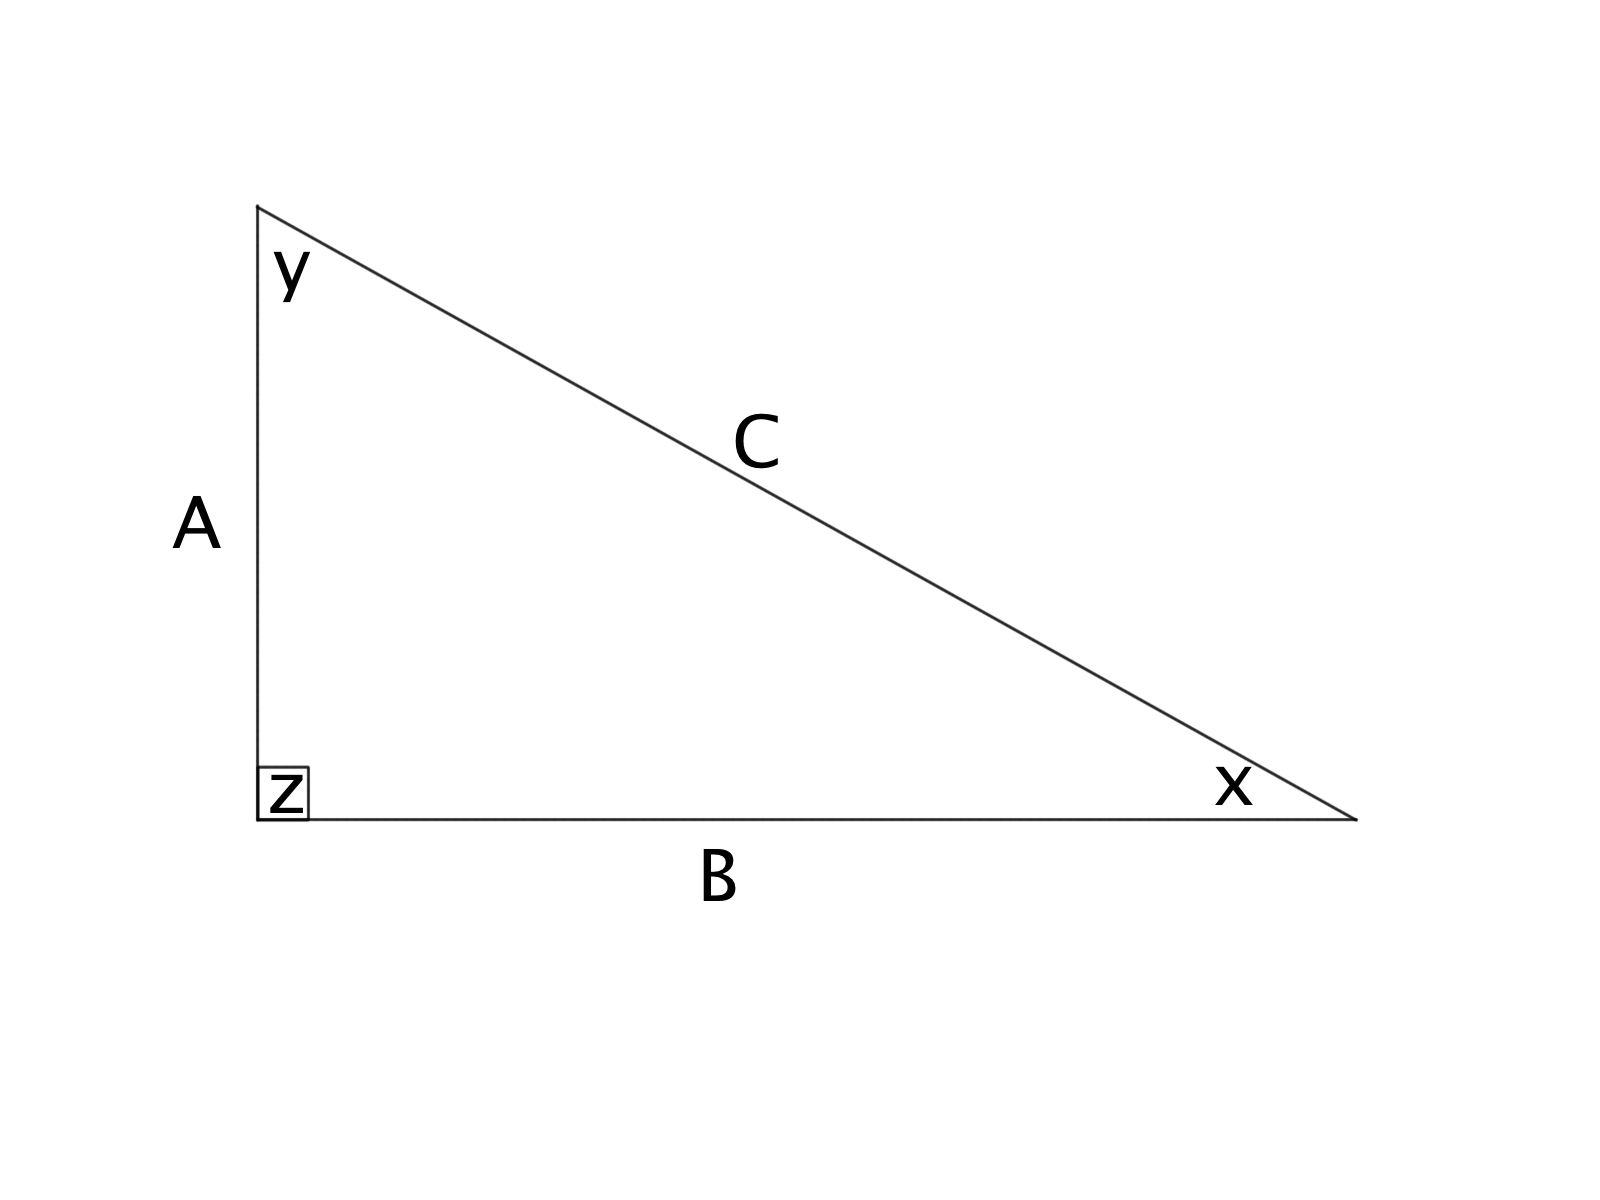
\includegraphics[width=5cm]{figures/triangle.jpg}
%    \caption[Placeholder]{Placeholder figure.}\label{fig:first}
%  \end{center}
%\end{figure}

%\begin{table}[h]                        
%  \begin{center}                          
%    \begin{tabular}{r|c|c}                  
%      \hline \hline                           
%      $(1,1)$ & $(1,2)$ & $(1,3)$\\           
%      \hline                                  
%      $(2,1)$ & $(2,2)$ & $(2,3)$\\           
%      \hline                                  
%      $(3,1)$ & $(3,2)$ & $(3,3)$\\
%      \hline \hline                           
%    \end{tabular}
%    \caption[Placeholder Table]{Placeholder table.}\label{tab:uno}
%  \end{center}
%\end{table}




%%%%%%%%%%%%%%%%%%%%%%%%%%%%%%%%%%%%%%% ACKNOWLEDGEMENTS %%%%%%%%%%%%%%%%%%%%%%%%%%%

\chapter*{Acknowledgements}

\thispagestyle{empty}

I wish to acknowledge the essential role my advisor Professor F. Zanasi has had in guiding me through the process of writing this thesis. He introduced me to applied category theory, to machine learning, and to the world of academic research, and I shall be forever grateful for it. I also wish to thank my family and my friends, who supported my throughout this journey and without whom all of this would not have been possible. To all of you, my most sincere gratitude.



\end{document}
